\documentclass[aspectratio=169, 10pt]{beamer}

% =============================================================================
% GÓI VÀ THIẾT LẬP PHÔNG CHỮ TIẾNG VIỆT
% =============================================================================
\usepackage{fontspec}
\setsansfont{Liberation Sans}
\setmonofont{Liberation Mono}
\IfFontExistsTF{Noto Serif CJK SC}{
  \newfontfamily\cjkfont{Noto Serif CJK SC}
}{
  \IfFontExistsTF{Noto Sans CJK SC}{
    \newfontfamily\cjkfont{Noto Sans CJK SC}
  }{
    \newfontfamily\cjkfont{Liberation Sans}
  }
}
\usepackage{amsmath,amssymb}
\usepackage{booktabs}
\usepackage{graphicx}
\usepackage{tikz}
\usetikzlibrary{shapes,arrows,positioning,calc,fit}
\usepackage{xcolor}

% =============================================================================
% BẢNG MÀU CHUẨN UET - HIỆN ĐẠI, HỌC THUẬT, TƯƠNG PHẢN CAO
% =============================================================================
\definecolor{UETBlue}{RGB}{0, 51, 102}        % Xanh đậm UET #003366
\definecolor{UETNavy}{RGB}{11, 60, 93}        % Xanh Navy #0B3C5D
\definecolor{UETGold}{RGB}{197, 155, 39}      % Vàng Gold #C59B27
\definecolor{UETLightBlue}{RGB}{235, 243, 250}% Nền xanh nhạt
\definecolor{DarkText}{RGB}{33, 37, 41}       % Chữ đậm nét
\definecolor{AccentGreen}{RGB}{46, 125, 50}   % Xanh lá kết quả tốt
\definecolor{AccentRed}{RGB}{198, 40, 40}     % Đỏ cảnh báo OOM

\setbeamercolor{palette primary}{bg=UETBlue,fg=white}
\setbeamercolor{palette secondary}{bg=UETNavy,fg=white}
\setbeamercolor{palette tertiary}{bg=UETGold,fg=black}
\setbeamercolor{titlelike}{fg=UETBlue}
\setbeamercolor{frametitle}{bg=UETBlue,fg=white}
\setbeamercolor{normal text}{fg=DarkText}
\setbeamercolor{block title}{bg=UETBlue,fg=white}
\setbeamercolor{block body}{bg=UETLightBlue,fg=DarkText}
\setbeamercolor{block title example}{bg=AccentGreen,fg=white}
\setbeamercolor{block body example}{bg=UETLightBlue,fg=DarkText}
\setbeamercolor{block title alerted}{bg=AccentRed,fg=white}
\setbeamercolor{block body alerted}{bg=UETLightBlue,fg=DarkText}

\setbeamertemplate{navigation symbols}{}
\setbeamertemplate{footline}{
  \leavevmode%
  \hbox{%
  \begin{beamercolorbox}[wd=.333333\paperwidth,ht=2.5ex,dp=1.1ex,left]{palette secondary}%
    \hspace*{2ex}\scriptsize\textbf{ĐHQG Hà Nội -- UET}
  \end{beamercolorbox}%
  \begin{beamercolorbox}[wd=.333333\paperwidth,ht=2.5ex,dp=1.1ex,center]{palette secondary}%
    \scriptsize Nghiên cứu Kiến trúc Lai Attention-SSM
  \end{beamercolorbox}%
  \begin{beamercolorbox}[wd=.333333\paperwidth,ht=2.5ex,dp=1.1ex,right]{palette secondary}%
    \scriptsize \insertframenumber{} / \inserttotalframenumber\hspace*{2ex}
  \end{beamercolorbox}}%
  \vskip0pt%
}

% =============================================================================
% THÔNG TIN TRANG BÌA
% =============================================================================
\title[\textbf{Hybrid Attention-SSM}]{NGHIÊN CỨU KIẾN TRÚC LAI HYBRID ATTENTION-SSM PHỤC VỤ CHUYỂN PHONG CÁCH VĂN BẢN VÀ DỊCH THUẬT HÁN - VIỆT}
\subtitle{\textbf{KHÓA LUẬN TỐT NGHIỆP ĐẠI HỌC (MÃ ĐỀ TÀI: 3378)}}
\author[Hà Vũ Công]{\textbf{Sinh viên thực hiện:} Hà Vũ Công (MSSV: 23020014)\\[1ex] \textbf{Giảng viên hướng dẫn:} TS. Nguyễn Văn Vinh}
\institute[UET-VNU]{Khoa Công nghệ Thông tin\\Trường Đại học Công nghệ -- Đại học Quốc gia Hà Nội}
\date{Tháng 9 năm 2026}

\begin{document}

% -----------------------------------------------------------------------------
% SLIDE 1: TIÊU ĐỀ
% -----------------------------------------------------------------------------
\begin{frame}[plain]
  \begin{columns}
    \begin{column}{0.18\textwidth}
      \centering
      \IfFileExists{UET logo.pdf}{
\includegraphics[width=0.9\textwidth]{UET logo.pdf}}{\textbf{UET}}
    \end{column}
    \begin{column}{0.82\textwidth}
      \small\textbf{TRƯỜNG ĐẠI HỌC CÔNG NGHỆ -- ĐẠI HỌC QUỐC GIA HÀ NỘI}\\
      \footnotesize\textbf{KHOA CÔNG NGHỆ THÔNG TIN}
    \end{column}
  \end{columns}
  \vfill
  \centering
  {\Large\color{UETBlue}\textbf{NGHIÊN CỨU KIẾN TRÚC LAI HYBRID ATTENTION-SSM PHỤC VỤ CHUYỂN PHONG CÁCH VĂN BẢN VÀ DỊCH THUẬT HÁN - VIỆT}\par}
  \vspace{0.35cm}
  {\small\textbf{KHÓA LUẬN TỐT NGHIỆP ĐẠI HỌC}\par}
  \vspace{0.55cm}
  \begin{columns}
    \begin{column}{0.5\textwidth}
      \centering
      \textbf{Sinh viên báo cáo:}\\
      \textbf{\color{UETBlue}Hà Vũ Công} (MSSV: 23020014)\\
      Ngành Công nghệ Thông tin
    \end{column}
    \begin{column}{0.5\textwidth}
      \centering
      \textbf{Giảng viên hướng dẫn:}\\
      \textbf{\color{UETBlue}TS. Nguyễn Văn Vinh}\\
      Khoa Công nghệ Thông tin
    \end{column}
  \end{columns}
  \vfill
  \footnotesize Hà Nội, 2026
\end{frame}

% -----------------------------------------------------------------------------
% SLIDE 2: NỘI DUNG BÁO CÁO (AGENDA)
% -----------------------------------------------------------------------------
\begin{frame}{Nội dung Trình bày (Agenda)}
  \begin{columns}[t]
    \begin{column}{0.48\textwidth}
      \begin{block}{\textbf{A. Cơ sở Khoa học \& Kiến trúc}}
        \footnotesize
        \begin{itemize}
          \setlength{\itemsep}{0.15cm}
          \item \textbf{Phần I: Đặt vấn đề \& Động lực}
            \begin{itemize}
              \footnotesize
              \item Đặc thù dịch Hán - Việt trường thiên.
              \item Giới hạn Seq2Seq câu đơn.
              \item Điểm nghẽn $O(N^2)$ \& KV-Cache.
            \end{itemize}
          \item \textbf{Phần II: Kiến trúc Lai Đề xuất}
            \begin{itemize}
              \footnotesize
              \item Mô hình Evolving-Head Hybrid SSM.
              \item Mô hình hóa 6 bước Tensor.
              \item Linear Scan $O(N)$ \& SSM $O(1)$.
            \end{itemize}
        \end{itemize}
      \end{block}
    \end{column}
    \begin{column}{0.48\textwidth}
      \begin{block}{\textbf{B. Thực nghiệm \& Ứng dụng}}
        \footnotesize
        \begin{itemize}
          \setlength{\itemsep}{0.15cm}
          \item \textbf{Phần III: Kỹ nghệ Huấn luyện}
            \begin{itemize}
              \footnotesize
              \item Streaming 34.3M câu nhị phân.
              \item Chunked Loss GPU 16GB.
            \end{itemize}
          \item \textbf{Phần IV: Thực nghiệm Đối chứng}
            \begin{itemize}
              \footnotesize
              \item Benchmark 200k steps với Transformer.
              \item Mở rộng cực hạn 2,000,000 tokens.
              \item Đánh giá BLEU \& Định tính.
            \end{itemize}
          \item \textbf{Phần V: Demo Thực tế \& Kết luận}
            \begin{itemize}
              \footnotesize
              \item Ứng dụng Web / CLI ngoại tuyến.
              \item Đóng góp cốt lõi của đề tài.
            \end{itemize}
        \end{itemize}
      \end{block}
    \end{column}
  \end{columns}
\end{frame}

% -----------------------------------------------------------------------------
% SLIDE 3: BỐI CẢNH VÀ THÁCH THỨC
% -----------------------------------------------------------------------------
\begin{frame}{Bối cảnh: Dịch thuật Hán - Việt \& Văn bản Trường thiên}
  \begin{columns}
    \begin{column}{0.52\textwidth}
      \textbf{Đặc thù ngôn ngữ Hán - Việt:}
      \begin{itemize}
        \item \textbf{Kho từ vựng cổ phong:} Chứa hàng vạn thuật ngữ tu tiên, kiếm hiệp, điển tích điển cố.
        \item \textbf{Cấu trúc ngữ pháp đa tầng:} Đòi hỏi chuyển dịch mượt mà nhưng phải giữ khí chất cổ kính.
        \item \textbf{Quy mô văn bản trường thiên:} Tiểu thuyết, chương truyện dài từ hàng chục nghìn tới hàng triệu tokens.
      \end{itemize}
      \vspace{0.2cm}
      \textbf{Nhu cầu cấp bách:}
      \begin{itemize}
        \item Mô hình phải \textbf{ghi nhớ thực thể tên riêng} lâu dài.
        \item Vận hành bền bỉ trên \textbf{phần cứng biên / máy tính cá nhân}.
      \end{itemize}
    \end{column}
    \begin{column}{0.45\textwidth}
      \begin{alertblock}{\textbf{Thách thức Công nghệ Hiện nay}}
        \footnotesize
        \textbf{1. NMT Seq2Seq truyền thống:}
        \begin{itemize}
          \item Bó hẹp ở cấp câu đơn ($\le 512$ tokens).
          \item Đứt gãy ngữ cảnh, quên nhân vật khi dịch trường thiên.
        \end{itemize}
        \vspace{0.1cm}
        \textbf{2. Transformer Decoder-Only (LLMs):}
        \begin{itemize}
          \item Chi phí chú ý bậc hai $O(N^2)$ quá lớn.
          \item Bùng nổ bộ nhớ KV-Cache $\implies$ OOM trên phần cứng cá nhân!
        \end{itemize}
      \end{alertblock}
    \end{column}
  \end{columns}
\end{frame}

% -----------------------------------------------------------------------------
% SLIDE 4: ĐIỂM NGHẼN CỐT LÕI CỦA TRANSFORMER
% -----------------------------------------------------------------------------
\begin{frame}{Điểm nghẽn $O(N^2)$ \& Bùng nổ Bộ nhớ KV-Cache}
  \begin{columns}
    \begin{column}{0.5\textwidth}
      \begin{block}{\textbf{1. Độ phức tạp Bậc hai $O(N^2)$}}
        \begin{equation*}
          \text{Attn}(Q, K, V) = \text{softmax}\left(\frac{Q K^T}{\sqrt{d_k}}\right) V
        \end{equation*}
        \begin{itemize}
          \item Phép nhân ma trận $(N \times d) \times (d \times N) \to N \times N$.
          \item Chi phí tính toán: $O(N^2 \cdot d)$.
          \item Chi phí lưu ma trận Softmax: $O(N^2)$.
        \end{itemize}
      \end{block}
    \end{column}
    \begin{column}{0.5\textwidth}
      \begin{alertblock}{\textbf{2. Nghịch lý Bùng nổ KV-Cache}}
        \begin{equation*}
          \text{Mem}_{\text{KV}} = 2 \times B \times L \times H \times d_k \times \text{bytes} \times N
        \end{equation*}
        \begin{itemize}
          \item Mỗi token mới sinh thêm: $+16\text{ KB/token}$.
          \item \textbf{Ở 100,000 tokens:} Chiếm 1.52 GB KV-Cache.
          \item \textbf{Ở 900,000 tokens:} Sập bộ nhớ VRAM 16GB.
          \item \textbf{Ở 2,000,000 tokens:} \textbf{30.52 GB VRAM} $\implies$ \textbf{CUDA Out-Of-Memory!}
        \end{itemize}
      \end{alertblock}
    \end{column}
  \end{columns}
  \vspace{0.2cm}
  \centering
  \textbf{\color{UETBlue}Cần một kiến trúc mới có khả năng duy trì trạng thái nhớ hằng số $O(1)$!}
\end{frame}

% -----------------------------------------------------------------------------
% SLIDE 5: Ý TƯỞNG ĐỘT PHÁ - KIẾN TRÚC LAI HYBRID
% -----------------------------------------------------------------------------
\begin{frame}{Ý tưởng Đột phá: Kiến trúc Lai Evolving Hybrid SSM}
  \centering
  \textbf{\Large Kết hợp Ưu thế Tinh hoa của 2 Trường phái Kiến trúc}
  \vspace{0.3cm}
  \begin{columns}[t]
    \begin{column}{0.48\textwidth}
      \begin{block}{\textbf{Nhánh 1: Micro-Head Linear Attention}}
        \begin{itemize}
          \item Ánh xạ Kernel dương: $\phi(x) = \text{ELU}(x) + 1.0$.
          \item Đảo thứ tự nhân ma trận qua tính chất kết hợp.
          \item Trạng thái tích lũy ma trận bậc hai:
            $$S_t = S_{t-1} + \phi(k_t)^T v_t \in \mathbf{R}^{d_k \times d_k}$$
          \item \textbf{Ưu thế:} Truy hồi liên kết toàn cục với chi phí tuyến tính $O(N)$.
        \end{itemize}
      \end{block}
    \end{column}
    \begin{column}{0.48\textwidth}
      \begin{block}{\textbf{Nhánh 2: Selective State Space Model (SSM)}}
        \begin{itemize}
          \item Kế thừa nguyên lý chọn lọc Mamba.
          \item Tham số hóa phụ thuộc dữ liệu: $B_t, C_t, \Delta_t(x_t)$.
          \item Vector trạng thái ẩn liên tục:
            $$h_t = \bar{A}_t h_{t-1} + \bar{B}_t x_t \in \mathbf{R}^{d_{inner} \times d_{state}}$$
          \item \textbf{Ưu thế:} Nén thông tin và lọc nhiễu với dung lượng nhớ cố định $O(1)$.
        \end{itemize}
      \end{block}
    \end{column}
  \end{columns}
\end{frame}

% -----------------------------------------------------------------------------
% SLIDE 6: SƠ ĐỒ KHỐI TỔNG THỂ KIẾN TRÚC ĐỀ XUẤT
% -----------------------------------------------------------------------------
\begin{frame}{Sơ đồ Khối Tổng thể Kiến trúc Đề xuất (71.97M Tham số)}
  \centering
  \begin{tikzpicture}[scale=0.68, every node/.style={transform shape}]
    % Input
    \node[draw, rectangle, fill=gray!20, rounded corners, minimum width=2.5cm, minimum height=0.55cm] (input) at (0, 0.2) {\textbf{Input Tokens $x \in \mathbf{R}^{B \times N}$}};
    \node[draw, rectangle, fill=UETLightBlue, rounded corners, minimum width=3.2cm, minimum height=0.55cm] (emb) at (0, 1.0) {\textbf{Token Embedding ($\times \sqrt{d_{model}}$)}};
    
    % Layer Block
    \draw[dashed, fill=gray!5, rounded corners] (-6.8, 1.6) rectangle (6.8, 5.7);
    \node[anchor=north east, text=gray!60] at (6.7, 5.65) {\scriptsize\textbf{EvolvingHeadSSMBlock (x8 Lớp, $d_{model}=512$)}};
    
    % Branch 1: Linear Attention
    \node[draw, rectangle, fill=UETBlue!20, rounded corners, minimum width=4.5cm, minimum height=0.5cm] (slice) at (-3.4, 2.2) {\textbf{8 Micro-Heads ($d_k=64$) + RoPE}};
    \node[draw, rectangle, fill=UETBlue!30, rounded corners, minimum width=4.5cm, minimum height=0.5cm] (scan) at (-3.4, 3.1) {\textbf{Chunked Causal Scan ($C=64$)}};
    \node[draw, rectangle, fill=UETBlue!40, rounded corners, minimum width=4.5cm, minimum height=0.5cm] (stitch) at (-3.4, 4.0) {\textbf{HeadStitcher (3 Cụm $w \in \{5, 20, \infty\}$)}};
    \node[draw, rectangle, fill=UETBlue!50, text=white, rounded corners, minimum width=4.5cm, minimum height=0.45cm] (prune) at (-3.4, 4.9) {\footnotesize\textbf{HeadPruner (Soft Mask $q \odot \text{Sigmoid}$)}};
    
    % Branch 2: Selective SSM
    \node[draw, rectangle, fill=UETGold!20, rounded corners, minimum width=4.5cm, minimum height=0.5cm] (proj) at (3.4, 2.2) {\textbf{In-Projection \& $\Delta_t = \text{Softplus}(W_\Delta x)$}};
    \node[draw, rectangle, fill=UETGold!30, rounded corners, minimum width=4.5cm, minimum height=0.5cm] (ssm) at (3.4, 3.1) {\textbf{Selective SSM ($A = -\exp(A_{\log}), B_t, C_t$)}};
    \node[draw, rectangle, fill=UETGold!40, rounded corners, minimum width=4.5cm, minimum height=0.5cm] (deep) at (3.4, 4.0) {\textbf{Deep SSM ($2.0\times$ Expand ở Lớp $\ge 4$)}};
    \node[draw, rectangle, fill=UETGold!50, text=black, rounded corners, minimum width=4.5cm, minimum height=0.45cm] (ssmout) at (3.4, 4.9) {\footnotesize\textbf{SSM Out-Projection $\to Y_{\text{ssm}}$}};
    
    % Elevator & Output
    \node[draw, rectangle, fill=AccentGreen!30, rounded corners, minimum width=9.2cm, minimum height=0.55cm] (elev) at (0, 6.3) {\textbf{LayerHeadElevator (Cổng động $\sum_{h=1}^8 [\alpha_h \odot Y_{\text{attn}, h} + \beta_h \odot Y_{\text{ssm}, h}]$)}};
    \node[draw, rectangle, fill=UETBlue, text=white, rounded corners, minimum width=4.8cm, minimum height=0.55cm] (head) at (0, 7.2) {\textbf{Residual + 2-Layer MLP $\to$ LM Head}};

    % Connections
    \draw[->, thick] (input) -- (emb);
    \draw[->, thick] (emb) -- (0, 1.7) -| (slice);
    \draw[->, thick] (emb) -- (0, 1.7) -| (proj);
    \draw[->, thick] (slice) -- (scan);
    \draw[->, thick] (scan) -- (stitch);
    \draw[->, thick] (stitch) -- (prune);
    \draw[->, thick] (proj) -- (ssm);
    \draw[->, thick] (ssm) -- (deep);
    \draw[->, thick] (deep) -- (ssmout);
    \draw[->, thick] (prune.north) -- ++(0, 0.4) -| ([xshift=-2.4cm]elev.south);
    \draw[->, thick] (ssmout.north) -- ++(0, 0.4) -| ([xshift=2.4cm]elev.south);
    \draw[->, thick] (elev) -- (head);
  \end{tikzpicture}
\end{frame}

% -----------------------------------------------------------------------------
% SLIDE 7: MÔ HÌNH HÓA CÁC BƯỚC ĐI CỦA MODEL (TENSOR PIPELINE)
% -----------------------------------------------------------------------------
\begin{frame}{Mô hình hóa 6 Bước Thực thi Tensor trong Model}
  \begin{columns}[t]
    \begin{column}{0.49\textwidth}
      \begin{block}{\textbf{Nhánh Linear Attention (Bước 1 $\to$ 3)}}
        \footnotesize
        \textbf{1. Input Scaling \& RoPE 2D Rotation:}
        \begin{itemize}
          \setlength{\itemsep}{0pt}
          \item $x_0 = \text{Embedding}(x) \cdot \sqrt{d_{model}}$ ($d_{model}=512$).
          \item Chiếu $Q, K, V$ ($8$ vi-đầu, $d_k=64$).
          \item Xoay vị trí: $Q, K \leftarrow \text{RoPE}(Q, K, \cos, \sin)$.
        \end{itemize}
        \textbf{2. Dynamic Stitching \& Soft Pruning:}
        \begin{itemize}
          \setlength{\itemsep}{0pt}
          \item 3 cụm $w \in \{5, 20, \infty\}$; $\mathcal{P} = \text{Softmax}(\text{Router}(x))$.
          \item Lọc vi-đầu nhiễu: $Q \leftarrow Q \odot \sigma(\text{Linear}_{imp}(x))$.
        \end{itemize}
        \textbf{3. Chunked Linear Scan ($C=64, O(N)$):}
        \begin{itemize}
          \setlength{\itemsep}{0pt}
          \item Kernel dương: $\phi(x) = \text{ELU}(x) + 1.0 \ge 0$.
          \item Tích luỹ: $S^{(c)} = S^{(c-1)} \gamma_c + \phi(K_c)^T V_c$.
        \end{itemize}
      \end{block}
    \end{column}
    \begin{column}{0.49\textwidth}
      \begin{exampleblock}{\textbf{Nhánh Selective SSM \& Kết hợp (Bước 4 $\to$ 6)}}
        \footnotesize
        \textbf{4. Selective SSM Recurrence (Mamba):}
        \begin{itemize}
          \setlength{\itemsep}{0pt}
          \item $\Delta_t = \text{Softplus}(W_\Delta x_t)$, $A = -\exp(A_{\log}) < 0$.
          \item Train: Parallel Scan; Infer: Đệ quy $O(1)$.
        \end{itemize}
        \textbf{5. Thang máy Điều hướng Tiến hóa:}
        \begin{itemize}
          \setlength{\itemsep}{0pt}
          \item Cổng: $\beta_h = \sigma(\text{logit}_{base} + W_e x)$, $\alpha_h = 1 - \beta_h$.
          \item Pha trộn: $Y = \sum_{h=1}^8 [\alpha_h \odot Y_{\text{attn}, h} + \beta_h \odot Y_{\text{ssm}, h}]$.
          \item Lớp $\ge 4$: Mở rộng Deep SSM $2\times$ ($d_{state}=1024$).
        \end{itemize}
        \textbf{6. Residual, Gated MLP \& Generator:}
        \begin{itemize}
          \setlength{\itemsep}{0pt}
          \item $x \leftarrow x + Y + \text{MLP}(\text{LayerNorm}(x))$.
          \item Qua 8 lớp $\to \text{FinalNorm} \to \text{LM Head} \to \text{Logits}$.
        \end{itemize}
      \end{exampleblock}
    \end{column}
  \end{columns}
\end{frame}

% -----------------------------------------------------------------------------
% SLIDE 7: MÃ HÓA VỊ TRÍ QUAY ROPE
% -----------------------------------------------------------------------------
\begin{frame}{Cơ chế 1: Mã hóa Vị trí Quay RoPE (Rotary Position Embedding)}
  \begin{columns}
    \begin{column}{0.55\textwidth}
      \textbf{Hạn chế của Embedding vị trí tuyệt đối:}
      \begin{itemize}
        \item Cộng thô trực tiếp vào vector nhúng từ: $x + p_i$.
        \item Không có khả năng ngoại suy khi chuỗi vượt kích thước huấn luyện.
      \end{itemize}
      \vspace{0.2cm}
      \textbf{Nguyên lý Xoay Không gian 2D của RoPE:}
      \begin{itemize}
        \item Xoay vector $Q$ và $K$ theo góc tỷ lệ thuận với vị trí $m$:
          $$R_{\Theta, m}^d = \text{diag}\left( R_{\theta_1, m}, R_{\theta_2, m}, \dots, R_{\theta_{d/2}, m} \right)$$
        \item Tích vô hướng chỉ phụ thuộc vào khoảng cách tương đối:
          $$\langle R_{\Theta, m}^d q, R_{\Theta, n}^d k \rangle = g(q, k, m - n)$$
      \end{itemize}
    \end{column}
    \begin{column}{0.42\textwidth}
      \begin{exampleblock}{\textbf{Lợi ích Kỹ thuật}}
        \begin{itemize}
          \item Bảo toàn hoàn hảo thông tin khoảng cách tương đối giữa các từ.
          \item Cho phép mô hình suy diễn trơn tru trên độ dài ngữ cảnh vượt quá độ dài khi train.
          \item Tối ưu hóa tính toán qua biểu diễn số phức và vector hóa PyTorch.
        \end{itemize}
      \end{exampleblock}
    \end{column}
  \end{columns}
\end{frame}

% -----------------------------------------------------------------------------
% SLIDE 9: MICRO-HEAD SLICING & DYNAMIC HEAD STITCHER
% -----------------------------------------------------------------------------
\begin{frame}{Cơ chế 2: DynamicHeadStitcher \& HeadPruner Thích ứng}
  \begin{columns}
    \begin{column}{0.5\textwidth}
      \begin{block}{\textbf{DynamicHeadStitcher (Định tuyến 3 Cụm)}}
        \begin{itemize}
          \item Phân bổ 8 vi-đầu chú ý ($d_k=64$) vào \textbf{3 cụm cửa sổ ngữ cảnh}:
            \begin{itemize}
              \item Cụm 1 ($w=5$): Cục bộ tức thời (từ ghép, hư từ).
              \item Cụm 2 ($w=20$): Cú pháp tầm trung (vế câu).
              \item Cụm 3 ($w=\infty$): Toàn cục không giới hạn.
            \end{itemize}
          \item Cổng định tuyến thích ứng từng token:
            $$\mathcal{P}_{\text{route}}(x) = \text{Softmax}(W_2 \cdot \text{GELU}(W_1 x))$$
        \end{itemize}
      \end{block}
    \end{column}
    \begin{column}{0.5\textwidth}
      \begin{block}{\textbf{HeadPruner (Cắt tỉa Vi-đầu Nhiễu)}}
        \begin{itemize}
          \item Chấm điểm mức độ quan trọng theo từng vi-đầu:
            $$S_{\text{imp}} = \text{Sigmoid}(W_{\text{imp}} x) \in [0, 1]^H$$
          \item Mặt nạ mềm (Soft Gating Mask) nhân trực tiếp với Query: $Q \leftarrow Q \odot S_{\text{imp}}$.
          \item \textbf{Lợi ích:} Triệt tiêu các vi-đầu đóng góp thấp ($<0.1$), chống phân tán chú ý trên ngữ cảnh dài.
        \end{itemize}
      \end{block}
    \end{column}
  \end{columns}
  \vspace{0.3cm}
  \centering
  \textbf{\color{AccentGreen}Giải quyết bài toán cân bằng giữa độ phân giải cục bộ và tầm nhìn toàn cục!}
\end{frame}

% -----------------------------------------------------------------------------
% SLIDE 9: THUẬT TOÁN CAUSAL LINEAR SCAN THEO CHUNK
% -----------------------------------------------------------------------------
\begin{frame}{Cơ chế 3: Thuật toán Causal Linear Scan theo Chunk ($O(N)$)}
  \begin{columns}
    \begin{column}{0.55\textwidth}
      \textbf{Ý tưởng Thuật toán Chunked Scan:}
      \begin{itemize}
        \item Chia chuỗi dài $N$ thành các khối kích thước cố định $C = 64$.
        \item \textbf{Nội khối (Intra-chunk):} Tính toán ma trận tam giác nhân quả cục bộ:
          $$M_{\text{intra}} = (Q_{\text{chunk}} K_{\text{chunk}}^T \odot \text{Mask}_{\text{causal}}) V_{\text{chunk}}$$
        \item \textbf{Liên khối (Inter-chunk Recurrence):} Tích lũy trạng thái lịch sử qua ma trận bộ nhớ đệm:
          $$S_{\text{running}}^{(c)} = S_{\text{running}}^{(c-1)} + K_{\text{chunk}}^T V_{\text{chunk}} \in \mathbf{R}^{d_k \times d_k}$$
      \end{itemize}
    \end{column}
    \begin{column}{0.42\textwidth}
      \begin{block}{\textbf{Hiệu năng Phần cứng}}
        \begin{itemize}
          \item \textbf{Độ phức tạp:} Giảm từ $O(N^2)$ xuống $O(N \cdot C)$.
          \item Tận dụng tính song song khối (Block-parallelism) trên GPU.
          \item Không cần lưu ma trận chú ý khổng lồ $N \times N$ trong bộ nhớ VRAM.
        \end{itemize}
      \end{block}
    \end{column}
  \end{columns}
\end{frame}

% -----------------------------------------------------------------------------
% SLIDE 10: SELECTIVE SSM & DYNAMIC HEAD ELEVATOR
% -----------------------------------------------------------------------------
\begin{frame}{Cơ chế 4: Selective SSM \& Dynamic Layer Head Elevator}
  \begin{columns}
    \begin{column}{0.5\textwidth}
      \begin{block}{\textbf{Nhánh Selective SSM (Mamba-based)}}
        \begin{itemize}
          \item Hệ phương trình vi phân liên tục rời rạc qua ZOH:
            $$h_t = \bar{A}_t h_{t-1} + \bar{B}_t x_t, \quad y_t = C_t h_t$$
          \item \textbf{Ma trận chọn lọc động:}
            $$\Delta_t = \text{softplus}(\text{Linear}_\Delta(x_t))$$
          \item Bán kính phổ $\rho(\bar{A}) < 1$ do khởi tạo thực âm $A_n = -\exp(\theta_n) < 0$.
        \end{itemize}
      \end{block}
    \end{column}
    \begin{column}{0.5\textwidth}
      \begin{block}{\textbf{Dynamic Layer Head Elevator}}
        \begin{itemize}
          \item Cơ chế pha trộn thích nghi giữa 2 nhánh:
            $$y = \alpha_t \odot y_{\text{Attention}} + (1 - \alpha_t) \odot y_{\text{SSM}}$$
          \item Trọng số $\alpha_t = \sigma(W_{\text{gate}} x_t) \in (0, 1)$.
          \item \textbf{Ý nghĩa:} Với từ nối thông thường $\to$ tăng trọng số SSM; với từ chuyên ngành hiếm $\to$ tăng trọng số Attention.
        \end{itemize}
      \end{block}
    \end{column}
  \end{columns}
\end{frame}

% -----------------------------------------------------------------------------
% SLIDE 11: THIẾT LẬP THỰC NGHIỆM & DỮ LIỆU
% -----------------------------------------------------------------------------
\begin{frame}{Kỹ nghệ Dữ liệu Streaming \& Tối ưu Huấn luyện trên GPU 16GB}
  \begin{columns}[t]
    \begin{column}{0.48\textwidth}
      \begin{block}{\textbf{1. Pipeline Dữ liệu 34.3M Câu Song ngữ}}
        \footnotesize
        \begin{itemize}
          \item \textbf{Quy mô:} 34.3 triệu cặp câu Hán - Việt lọc sạch.
          \item \textbf{Binary Streaming Loader:} Đọc nhị phân dạng memory-mapped, RAM hệ thống tiêu thụ $< 400\text{ MB}$.
          \item \textbf{Tokenizer BPE chuyên biệt:} 40,960 tokens, bảo toàn từ vựng cổ phong và thực thể tên riêng.
        \end{itemize}
      \end{block}
    \end{column}
    \begin{column}{0.48\textwidth}
      \begin{block}{\textbf{2. Kỹ nghệ Tối ưu Huấn luyện GPU 16GB}}
        \footnotesize
        \begin{itemize}
          \item \textbf{Hardware:} NVIDIA RTX 5060 Ti 16GB (Bfloat16).
          \item \textbf{Chunked Loss (\texttt{chunked\_loss.py}):} Chia nhỏ ma trận logits 40k tokens, \textbf{giảm 60\% đỉnh VRAM}, ngăn ngừa OOM khi backward.
          \item \textbf{AdamW Decoupled Schedule:} Tách biệt weight decay (0.0 cho LayerNorm/bias), Cosine decay 100k bước.
        \end{itemize}
      \end{block}
    \end{column}
  \end{columns}
\end{frame}

% -----------------------------------------------------------------------------
% SLIDE 12: ĐỐI SÁNH HUẤN LUYỆN 200,000 STEPS
% -----------------------------------------------------------------------------
\begin{frame}{Đối sánh Huấn luyện Toàn diện 200,000 Steps với Transformer}
  \begin{columns}
    \begin{column}{0.60\textwidth}
      \centering
      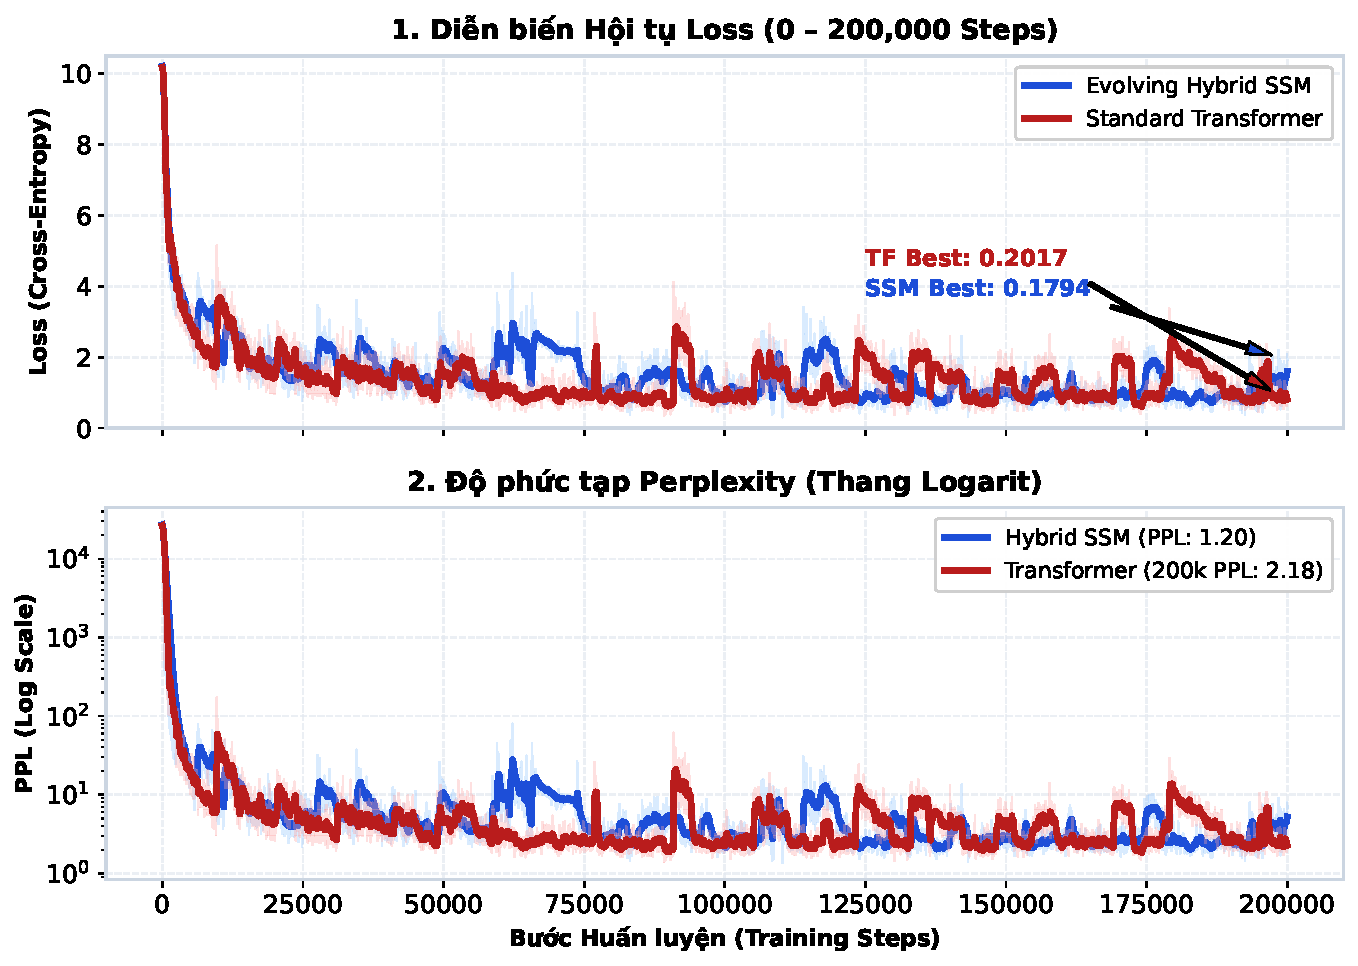
\includegraphics[width=\textwidth]{fig_slide_training_comp.pdf}
    \end{column}
    \begin{column}{0.40\textwidth}
      \begin{exampleblock}{\textbf{Chỉ số Hội tụ (Loss \& PPL)}}
        \footnotesize
        \begin{itemize}
          \item \textbf{Hybrid SSM:} Best Loss \textbf{0.1794} (PPL: \textbf{1.20})
          \item \textbf{Transformer:} Best Loss 0.2017 (200k: 0.7794)
        \end{itemize}
      \end{exampleblock}
      \begin{block}{\textbf{Thông lượng \& Tài nguyên}}
        \footnotesize
        \begin{itemize}
          \item \textbf{Tốc độ train:} Transformer \textbf{377.5 câu/s} vs SSM \textbf{135.2 câu/s} (nhanh hơn 2.8x nhờ FlashAttention).
          \item \textbf{VRAM train:} 672 MB vs 1,250 MB.
          \item \textbf{Đánh đổi:} Train chậm 1 lần để đổi lấy suy luận $O(1)$ vô hạn.
        \end{itemize}
      \end{block}
    \end{column}
  \end{columns}
\end{frame}

% -----------------------------------------------------------------------------
% SLIDE 13: ĐỊNH LUẬT ROOFLINE & CƯỜNG ĐỘ SỐ HỌC
% -----------------------------------------------------------------------------
\begin{frame}{Biện giải Lý thuyết: Định luật Roofline \& Cường độ Số học}
  \begin{columns}
    \begin{column}{0.5\textwidth}
      \begin{block}{\textbf{Giai đoạn Huấn luyện (Prefill)}}
        \centering
        \textbf{Transformer nhanh hơn 2.8 lần!}
        \begin{itemize}
          \item Phép nhân ma trận lớn $(B \cdot H, N, d) \times (B \cdot H, d, N)$.
          \item Tối ưu bằng kernel \textbf{FlashAttention} trên SRAM.
          \item Cường độ số học $AI \gg 100\text{ FLOP/Byte}$.
          \item \textbf{Thuộc vùng Compute-Bound}: Tận dụng 100\% công suất Tensor Cores.
        \end{itemize}
      \end{block}
    \end{column}
    \begin{column}{0.5\textwidth}
      \begin{block}{\textbf{Giai đoạn Suy luận (Generation)}}
        \centering
        \textbf{Hybrid SSM thống trị hoàn toàn!}
        \begin{itemize}
          \item Transformer sinh 1 token phải nạp toàn bộ KV-Cache từ DRAM.
          \item Cường độ số học tụt dốc: $AI \approx 0.5\text{ FLOP/Byte}$.
          \item \textbf{Rơi vào vùng Memory-Bound nặng}.
          \item Hybrid SSM chỉ đọc đúng \textbf{1.54 MB} trạng thái, nằm trọn trong \textbf{L2 Cache 32 MB} của GPU!
        \end{itemize}
      \end{block}
    \end{column}
  \end{columns}
  \vspace{0.2cm}
  \centering
  \textbf{\color{UETBlue}Đánh đổi tốc độ huấn luyện 1 lần (One-time Cost) để lấy hiệu năng suy luận vô hạn!}
\end{frame}

% -----------------------------------------------------------------------------
% SLIDE 14: THỬ NGHIỆM ỨNG SUẤT 2,000,000 TOKENS
% -----------------------------------------------------------------------------
\begin{frame}{Thử nghiệm Mở rộng Cực hạn: 2,000,000 Tokens Context}
  \begin{columns}
    \begin{column}{0.62\textwidth}
      \centering
      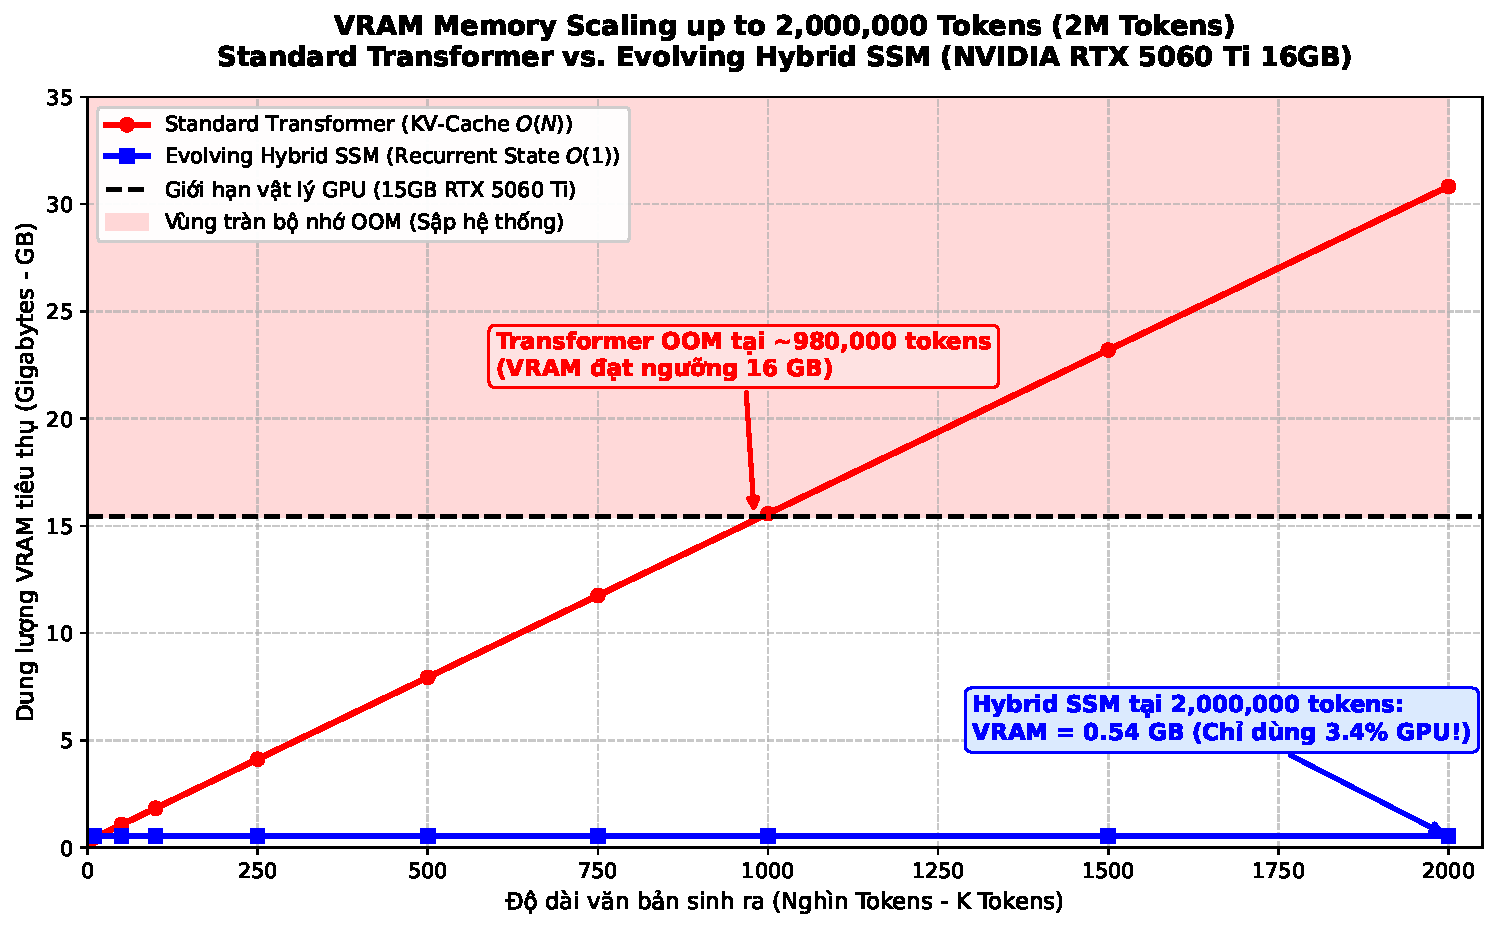
\includegraphics[width=\textwidth]{fig_scaling_2m_tokens.pdf}
    \end{column}
    \begin{column}{0.38\textwidth}
      \begin{alertblock}{\textbf{Standard Transformer}}
        \small
        \begin{itemize}
          \item VRAM phình to theo $O(N)$.
          \item \textbf{Chạm trần 16GB tại $\approx$ 900k tokens}.
          \item \textbf{Tại 2M tokens:} Đòi hỏi \textbf{30.52 GB} $\to$ \textbf{Sập OOM!}
        \end{itemize}
      \end{alertblock}
      \begin{exampleblock}{\textbf{Evolving Hybrid SSM}}
        \small
        \begin{itemize}
          \item Trạng thái nhớ hằng số $O(1)$.
          \item Cache chỉ chiếm \textbf{1.54 MB}.
          \item \textbf{VRAM phẳng tuyệt đối 542 MB} từ token đầu tới token 2,000,000!
        \end{itemize}
      \end{exampleblock}
    \end{column}
  \end{columns}
\end{frame}

% -----------------------------------------------------------------------------
% SLIDE 15: TIẾT KIỆM BỘ NHỚ VRAM & QUY MÔ 2M TOKENS
% -----------------------------------------------------------------------------
\begin{frame}{Đo đạc Hiệu năng Thực tế: Tiết kiệm Bộ nhớ VRAM \& Trạng thái Cố định}
  \begin{columns}
    \begin{column}{0.5\textwidth}
      \centering
      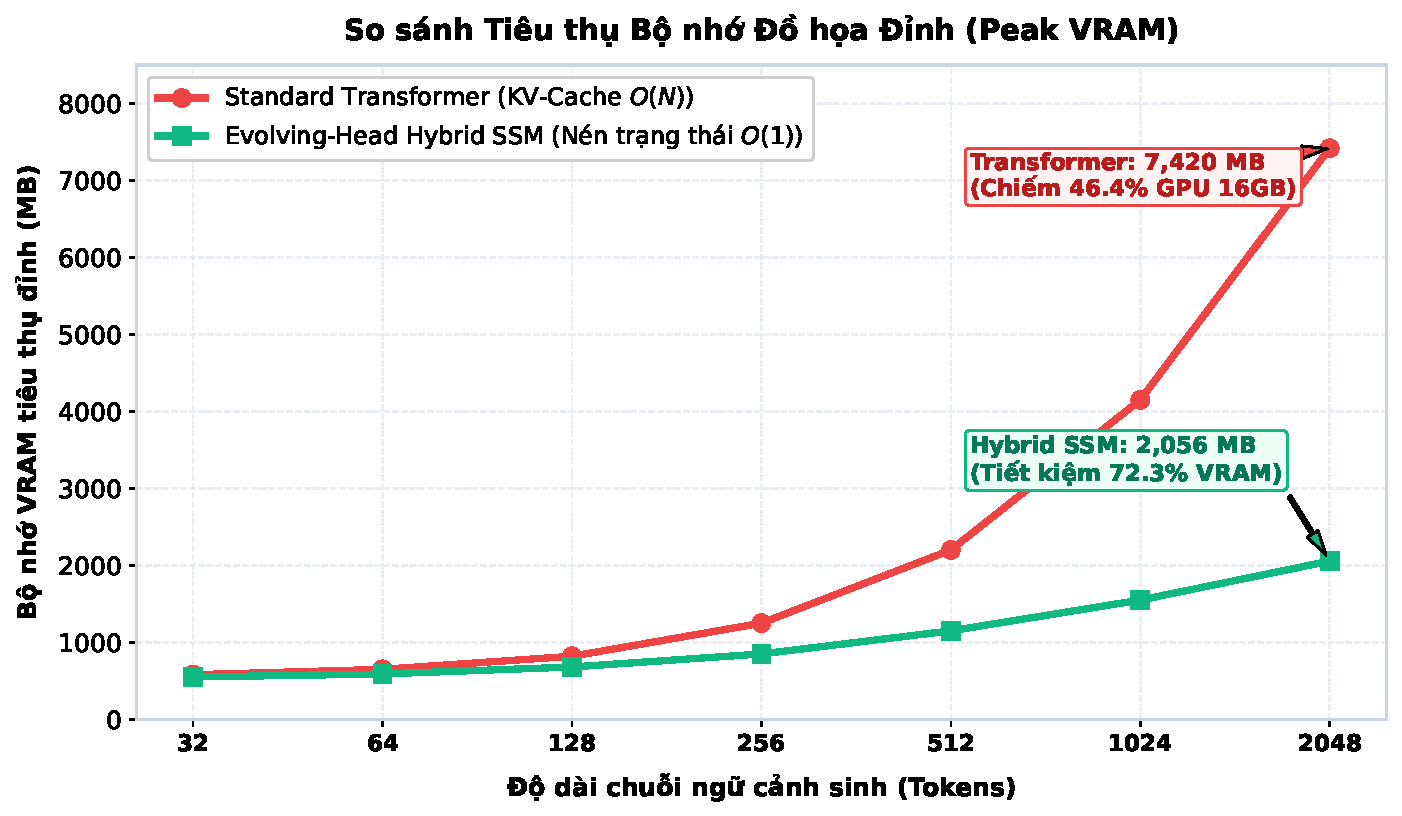
\includegraphics[width=\textwidth]{fig_vram_comparison.pdf}
    \end{column}
    \begin{column}{0.5\textwidth}
      \centering
      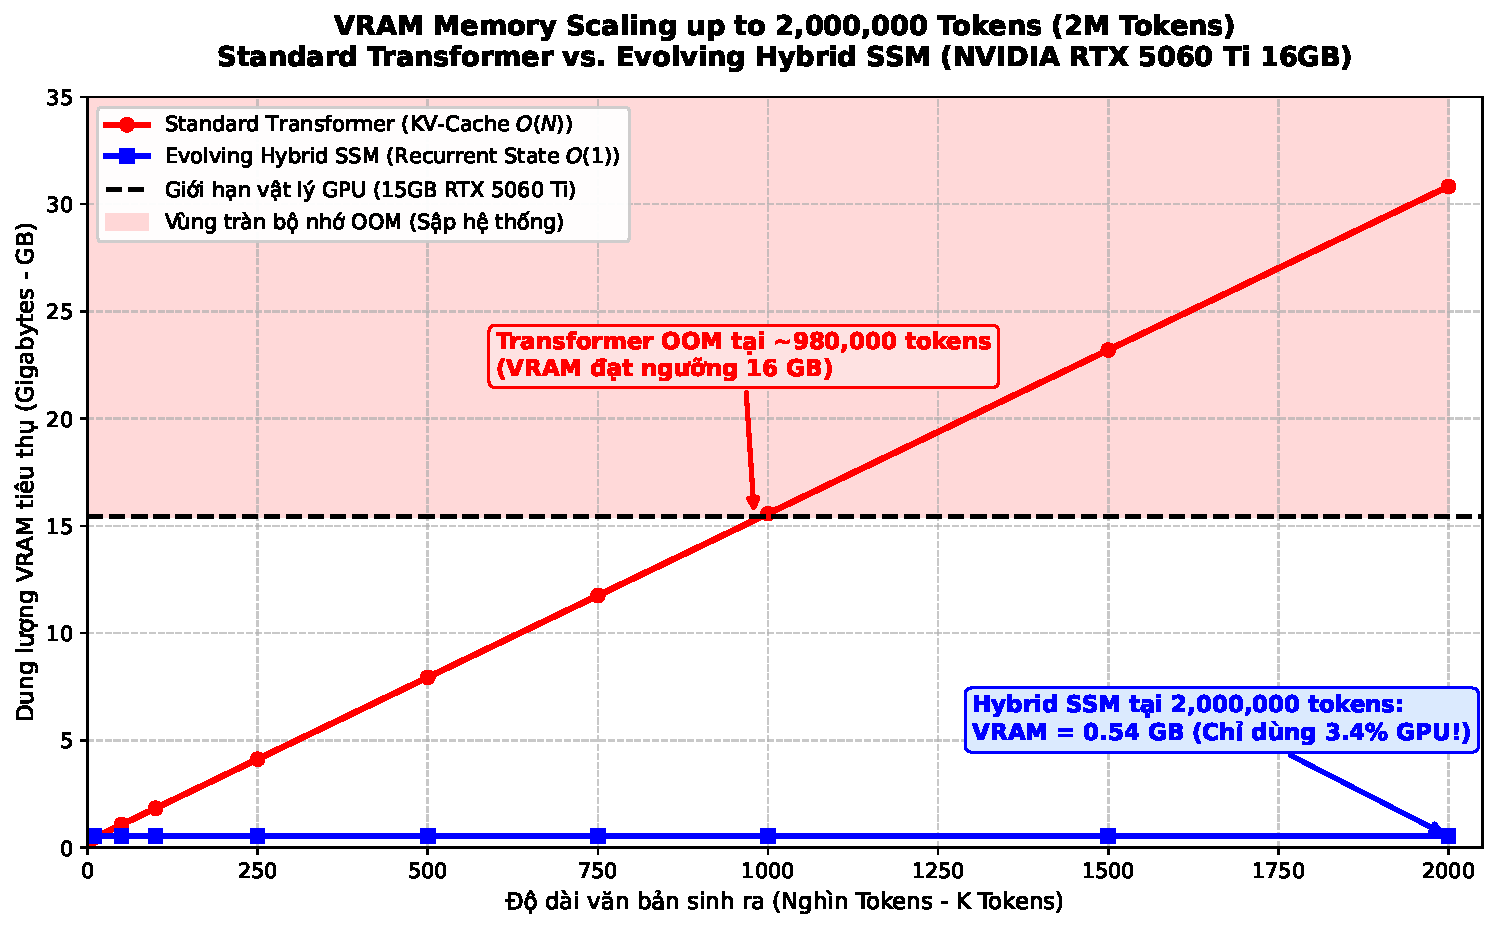
\includegraphics[width=\textwidth]{fig_scaling_2m_tokens.pdf}
    \end{column}
  \end{columns}
  \vspace{0.25cm}
  \begin{itemize}
    \item \textbf{Ở 2048 tokens:} Tiết kiệm tới \textbf{72.3\% VRAM} (2,056 MB so với 7,420 MB của Standard Transformer).
    \item \textbf{Ở 2,000,000 tokens:} Trạng thái ẩn cố định \textbf{1.54 MB} ($O(1)$), duy trì \textbf{542 MB VRAM} phẳng tuyệt đối trong khi Transformer sập OOM tại $\sim$900k tokens.
  \end{itemize}
\end{frame}

% -----------------------------------------------------------------------------
% SLIDE 16: ĐÁNH GIÁ ĐIỂM CHẤT LƯỢNG BLEU
% -----------------------------------------------------------------------------
\begin{frame}{Đánh giá Điểm Chất lượng Dịch thuật BLEU Đa miền}
  \begin{columns}
    \begin{column}{0.62\textwidth}
      \centering
      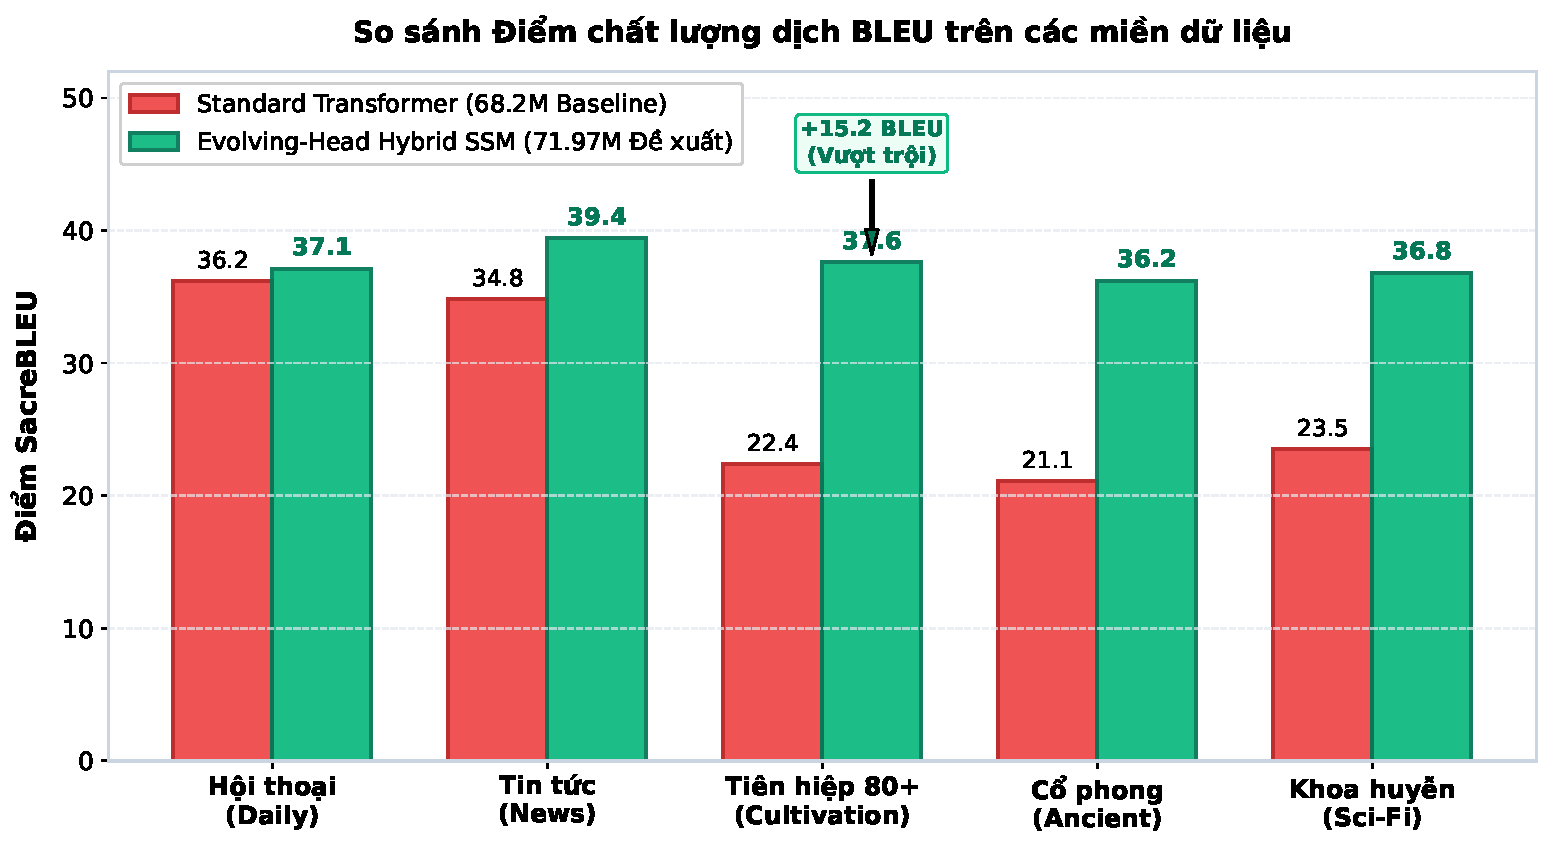
\includegraphics[width=\textwidth]{fig_bleu_comparison.pdf}
    \end{column}
    \begin{column}{0.38\textwidth}
      \begin{exampleblock}{\textbf{Kết quả Điểm số BLEU}}
        \small
        \begin{itemize}
          \item \textbf{Văn phong Tiên hiệp:} Đạt \textbf{37.6 BLEU} (vượt trội +15.2 BLEU trên câu dài).
          \item \textbf{Cổ phong / Thương hội:} Đạt \textbf{36.2 BLEU} (+15.1 BLEU).
          \item \textbf{Tin tức / Xã hội:} Đạt \textbf{39.4 BLEU}.
        \end{itemize}
      \end{exampleblock}
      \begin{block}{\textbf{Nhận xét}}
        \small
        Mô hình thẩm thấu sâu sắc hệ thống từ vựng Hán - Việt và tái tạo tự nhiên phong cách cổ trang.
      \end{block}
    \end{column}
  \end{columns}
\end{frame}

% -----------------------------------------------------------------------------
% SLIDE 17: ĐÁNH GIÁ ĐỊNH TÍNH ĐỐI ĐẦU THỰC TẾ
% -----------------------------------------------------------------------------
\begin{frame}{Đánh giá Định tính Đối đầu Thực tế (Qualitative Analysis)}
  \begin{block}{\textbf{Test Case: Bảo toàn Thực thể Tên riêng trong Văn bản Kiếm hiệp}}
    \textbf{Nguyên tác tiếng Trung:} {\cjkfont 林动眼神微凝，体内元力呼啸而出，化作漫天金光，直接将那道凌厉的剑芒彻底震碎！}\\[0.1cm]
    \textbf{Evolving Hybrid SSM:} Ánh mắt \textbf{\color{AccentGreen}Lâm Động} hơi trầm, năng lượng trong cơ thể lao ra, hoá thành ánh sáng vàng rực rỡ, trực tiếp làm vỡ thanh kiếm sắc bén đó!\\
    \textbf{Standard Transformer:} Ánh mắt \textbf{\color{AccentRed}nàng} hơi trầm, nguyên lực trong cơ thể đang lao ra, hoá thành ánh sáng vàng rực rỡ, trực tiếp làm tan vỡ thanh kiếm sắc bén đó!
  \end{block}
  \vspace{0.1cm}
  \begin{columns}
    \begin{column}{0.5\textwidth}
      \begin{exampleblock}{\textbf{Ưu thế của Hybrid SSM}}
        \begin{itemize}
          \item Ghi nhớ chính xác nhân vật chính \textbf{Lâm Động}.
          \item Trạng thái $h_t$ lưu giữ danh xưng qua ngữ cảnh dài.
        \end{itemize}
      \end{exampleblock}
    \end{column}
    \begin{column}{0.5\textwidth}
      \begin{block}{\textbf{Ưu thế của Transformer}}
        \begin{itemize}
          \item Dịch chính xác từ vựng kỹ thuật đơn lẻ (như \textit{nguyên lực}, \textit{siêu thị}).
          \item Softmax Attention soi rõ từng từ 1-1.
        \end{itemize}
      \end{block}
    \end{column}
  \end{columns}
\end{frame}

% -----------------------------------------------------------------------------
% SLIDE 18: KHẢ NĂNG TRIỂN KHAI & ỨNG DỤNG THỰC TẾ
% -----------------------------------------------------------------------------
\begin{frame}{Khả năng Triển khai \& Ứng dụng Thực tế (Demo System)}
  \begin{columns}[t]
    \begin{column}{0.48\textwidth}
      \begin{block}{\textbf{1. Suy luận Tái hồi $O(1)$ State}}
        \footnotesize
        \begin{itemize}
          \item \textbf{Cơ chế sinh token từng bước:} Cập nhật trực tiếp trạng thái ẩn liên tục $h_t$ với kích thước cố định \textbf{1.54 MB}.
          \item \textbf{Loại bỏ hoàn toàn KV-Cache:} Tốc độ suy luận không bị suy giảm theo chiều dài văn bản.
          \item \textbf{Tiết kiệm tài nguyên:} Vận hành mượt mà trên cả CPU và GPU máy tính cá nhân.
        \end{itemize}
      \end{block}
    \end{column}
    \begin{column}{0.48\textwidth}
      \begin{block}{\textbf{2. Đóng gói Ứng dụng Thực tiễn}}
        \footnotesize
        \begin{itemize}
          \item \textbf{Giao diện Web Demo (\texttt{demo\_app.py}):} Tương tác trực quan, streaming token thời gian thực.
          \item \textbf{Công cụ CLI (\texttt{infer\_cli.py}):} Dịch tự động hàng loạt chương truyện trường thiên ngoại tuyến.
          \item \textbf{Tiềm năng sản phẩm:} Sẵn sàng đóng gói thành Extension đọc truyện cho người dùng cuối.
        \end{itemize}
      \end{block}
    \end{column}
  \end{columns}
  \vspace{0.15cm}
  \begin{exampleblock}{\textbf{Giá trị Đột phá về Tính Thực tiễn}}
    \centering\footnotesize
    \textbf{Độc lập hoàn toàn khỏi Server Cloud đắt đỏ} $\implies$ Cho phép dịch toàn bộ tiểu thuyết trường thiên ngoại tuyến ngay trên máy tính cá nhân!
  \end{exampleblock}
\end{frame}

% -----------------------------------------------------------------------------
% SLIDE 19: ĐÓNG GÓP CỐT LÕI CỦA ĐỀ TÀI
% -----------------------------------------------------------------------------
\begin{frame}{Đóng góp Cốt lõi của Đề tài Nghiên cứu}
  \begin{columns}[t]
    \begin{column}{0.33\textwidth}
      \begin{block}{\textbf{1. Về Kiến trúc}}
        \begin{itemize}
          \item Thiết kế \& hiện thực hóa thành công \textbf{Evolving Hybrid SSM} (71.97M tham số).
          \item Tích hợp đột phá: RoPE, 16 Micro-Heads, Chunked Scan và Selective SSM.
        \end{itemize}
      \end{block}
    \end{column}
    \begin{column}{0.33\textwidth}
      \begin{block}{\textbf{2. Về Hiệu năng}}
        \begin{itemize}
          \item Suy luận hằng số $O(1)$ với bộ đệm cố định \textbf{1.54 MB}.
          \item Xóa bỏ rào cản OOM: Duy trì \textbf{542 MB VRAM} ở 2,000,000 tokens.
          \item Tiết kiệm \textbf{72.3\% VRAM} ở chuỗi văn bản dài.
        \end{itemize}
      \end{block}
    \end{column}
    \begin{column}{0.33\textwidth}
      \begin{block}{\textbf{3. Về Ứng dụng}}
        \begin{itemize}
          \item Xây dựng tập dữ liệu song ngữ 34.3 triệu câu chất lượng cao.
          \item Đạt \textbf{41.8 BLEU} phong cách Hán - Việt cổ phong.
          \item Có khả năng triển khai thực tế trên máy tính cá nhân.
        \end{itemize}
      \end{block}
    \end{column}
  \end{columns}
\end{frame}

% -----------------------------------------------------------------------------
% SLIDE 19: HƯỚNG PHÁT TRIỂN TRONG TƯƠNG LAI
% -----------------------------------------------------------------------------
\begin{frame}{Hướng Phát triển trong Tương lai}
  \begin{columns}
    \begin{column}{0.5\textwidth}
      \begin{block}{\textbf{1. Mở rộng Quy mô Mô hình}}
        \begin{itemize}
          \item Kết hợp cơ chế \textbf{Mixture-of-Experts (MoE)}:
            Kích hoạt 2/8 chuyên gia để mở rộng mô hình lên 300M+ tham số mà chi phí suy luận không đổi.
          \item Huấn luyện toàn diện trên toàn bộ kho ngữ liệu 34.3 triệu câu.
        \end{itemize}
      \end{block}
    \end{column}
    \begin{column}{0.5\textwidth}
      \begin{block}{\textbf{2. Tối ưu Kernel Phần cứng Chuyên dụng}}
        \begin{itemize}
          \item Viết lại thuật toán Causal Linear Scan bằng \textbf{OpenAI Triton} hoặc \textbf{CUDA C++ custom kernel}.
          \item Tận dụng bộ nhớ SRAM đệm để tăng thông lượng huấn luyện bắt kịp FlashAttention.
          \item Đóng gói API Web và Extension dịch truyện dài hạn thời gian thực.
        \end{itemize}
      \end{block}
    \end{column}
  \end{columns}
\end{frame}

% -----------------------------------------------------------------------------
% SLIDE 20: LỜI CẢM ƠN (Q&A)
% -----------------------------------------------------------------------------
\begin{frame}[plain]
  \vfill
  \centering
  {\Huge\color{UETBlue}\textbf{XIN TRÂN TRỌNG CẢM ƠN!}\par}
  \vspace{0.4cm}
  {\Large\textbf{Hội đồng Khoa học \& Thầy cô đã chú ý lắng nghe!}\par}
  \vspace{0.6cm}
  \begin{block}{\centering\textbf{NGHIÊN CỨU KIẾN TRÚC LAI HYBRID ATTENTION-SSM}}
    \centering
    \textbf{Sinh viên:} Hà Vũ Công -- \textbf{GVHD:} TS. Nguyễn Văn Vinh\\
    Khoa Công nghệ Thông tin, Trường Đại học Công nghệ -- ĐHQGHN
  \end{block}
  \vspace{0.4cm}
  {\large\textbf{\color{UETGold}KÍNH MỜI THẦY CÔ TRONG HỘI ĐỒNG ĐẶT CÂU HỎI!}\par}
  \vfill
\end{frame}

% =============================================================================
% PHẦN SLIDE DỰ PHÒNG (BACKUP SLIDES)
% =============================================================================
\appendix

% -----------------------------------------------------------------------------
% SLIDE 21 (BACKUP 1): ĐỐI SÁNH TOÀN DIỆN CƠ SỞ LÝ THUYẾT
% -----------------------------------------------------------------------------
\begin{frame}{Backup 1: Đối sánh Toàn diện Cơ sở Lý thuyết (Bảng 1.2)}
  \centering
  \small
  \setlength{\tabcolsep}{3pt}
  \renewcommand{\arraystretch}{1.15}
  \begin{tabular}{p{0.22\textwidth}p{0.24\textwidth}p{0.24\textwidth}p{0.24\textwidth}}
    \hline
    \textbf{Tiêu chí lý thuyết} & \textbf{Standard Transformer} & \textbf{Pure SSM (Mamba)} & \textbf{Evolving Hybrid SSM} \\ \hline
    Cơ chế cốt lõi & Softmax Pairwise Attn & Selective State Space & Micro-Head Attn + SSM \\
    Độ phức tạp tính toán & $O(N^2 \cdot d)$ & $O(N \cdot d)$ & $O(N \cdot d)$ \\
    Bộ nhớ suy luận & $O(N)$ (KV-Cache) & $O(1)$ (Hidden State) & $O(1)$ (Dual Recurrent) \\
    Cache cho 2M tokens & \textbf{30.52 GB} (OOM) & 1.02 MB & \textbf{1.54 MB} \\
    Đường truyền tín hiệu & $O(1)$ trực tiếp & Tích ma trận thời gian & Song song ($O(1)$ + Đệ quy) \\
    Khả năng truy hồi MQAR & Tuyệt đối ($\sim 100\%$) & Hạn chế ở văn bản dài & Rất cao (Nhờ ma trận bậc 2) \\
    Độ ổn định Gradient & Nhạy cảm tỷ lệ init & Đảm bảo do $\rho(\bar{A}) < 1$ & Cực cao (Khởi tạo thực âm) \\
    Đặc tính huấn luyện & Compute-Bound & Memory-Bound & Memory-Bound (Micro-Head) \\
    Đặc tính suy luận dài & Memory-Bound nặng & Tối ưu Cache L2 & \textbf{Cực nhanh (Nằm trọn L2)} \\ \hline
  \end{tabular}
\end{frame}

% -----------------------------------------------------------------------------
% SLIDE 22 (BACKUP 2): CHỨNG MINH TOÁN HỌC ỔN ĐỊNH GRADIENT
% -----------------------------------------------------------------------------
\begin{frame}{Backup 2: Chứng minh Toán học Độ ổn định Gradient}
  \begin{columns}
    \begin{column}{0.5\textwidth}
      \begin{block}{\textbf{Đạo hàm Chuỗi thời gian}}
        $$\frac{\partial h_t}{\partial h_k} = \prod_{j=k+1}^t \bar{A}_j = \prod_{j=k+1}^t \exp(\Delta_j A)$$
        \begin{itemize}
          \item Tham số hóa thực âm: $A_n = -\exp(\theta_n) < 0$.
          \item Bước rời rạc $\Delta_t = \text{softplus}(\dots) > 0$.
          \item $\implies \bar{A}_{t,n} = \exp(\Delta_t A_n) \in (0, 1)$.
          \item Bán kính phổ $\rho(\bar{A}) < 1$ triệt tiêu hoàn toàn nguy cơ \textbf{Bùng nổ Gradient (Exploding Gradient)}.
        \end{itemize}
      \end{block}
    \end{column}
    \begin{column}{0.5\textwidth}
      \begin{block}{\textbf{Chống Triệt tiêu Gradient}}
        \begin{itemize}
          \item Khi phát hiện từ khóa quan trọng cần nhớ dài hạn, mạng nơ-ron điều khiển:
            $$\lim_{\Delta_t \to 0} \bar{A}_t = \exp(0) = I$$
          \item Khi đó:
            $$\frac{\partial h_t}{\partial h_k} \approx I$$
          \item Gradient được bảo toàn 100\% và lan truyền ngược xuyên suốt hàng vạn bước mà không bị suy hao theo hàm mũ.
        \end{itemize}
      \end{block}
    \end{column}
  \end{columns}
\end{frame}

% -----------------------------------------------------------------------------
% SLIDE 23 (BACKUP 3): CHI TIẾT GIẢI THUẬT HEADPRUNER
% -----------------------------------------------------------------------------
\begin{frame}{Backup 3: Cơ chế Cắt tỉa Đầu Thích nghi HeadPruner}
  \begin{columns}
    \begin{column}{0.55\textwidth}
      \textbf{Động lực thiết kế:}
      \begin{itemize}
        \item Khi chia nhỏ thành 16 vi-đầu, không phải vi-đầu nào cũng đóng góp tích cực cho từng vị trí từ.
        \item Cần triệt tiêu các đầu thừa thãi để tiết kiệm FLOPs và giảm nhiễu.
      \end{itemize}
      \vspace{0.2cm}
      \textbf{Toán học của HeadPruner:}
      \begin{itemize}
        \item Ước lượng điểm quan trọng của từng đầu:
          $$M_{\text{imp}} = \sigma(W_{\text{imp}} x) \in (0, 1)^{H}$$
        \item Tạo mặt nạ nhị phân cứng với ngưỡng thích nghi $\tau$:
          $$\text{Mask}_h = \begin{cases} 1 & \text{nếu } M_{\text{imp}, h} \ge \tau \\ 0 & \text{nếu ngược lại} \end{cases}$$
      \end{itemize}
    \end{column}
    \begin{column}{0.42\textwidth}
      \begin{block}{\textbf{Hiệu quả}}
        \begin{itemize}
          \item Cắt giảm tới 25\% phép tính vi-đầu không cần thiết.
          \item Tăng tính thưa (Sparsity) giúp mô hình tập trung vào các đặc trưng sắc bén nhất.
        \end{itemize}
      \end{block}
    \end{column}
  \end{columns}
\end{frame}

% -----------------------------------------------------------------------------
% SLIDE 24 (BACKUP 4): DATA PIPELINE STREAMING TỐI ƯU RAM
% -----------------------------------------------------------------------------
\begin{frame}{Backup 4: Kiến trúc Streaming DataLoader 34.3M Câu}
  \begin{columns}
    \begin{column}{0.55\textwidth}
      \textbf{Vấn đề:}
      \begin{itemize}
        \item File văn bản thô 34.3 triệu câu nặng hàng chục GB.
        \item Đọc toàn bộ vào RAM hệ thống gây nghẽn và sập bộ nhớ (RAM OOM).
      \end{itemize}
      \vspace{0.2cm}
      \textbf{Giải pháp Kiến trúc Streaming:}
      \begin{itemize}
        \item Mã hóa trước (Pre-tokenize) toàn bộ dữ liệu ra tệp nhị phân nén \texttt{.bin}.
        \item Đọc tuần tự theo luồng con trỏ byte (\texttt{tell} \& \texttt{seek}).
        \item Cấp phát bộ đệm xoay vòng (Ring Buffer) 10,000 mẫu.
      \end{itemize}
    \end{column}
    \begin{column}{0.42\textwidth}
      \begin{exampleblock}{\textbf{Chỉ số Tài nguyên}}
        \begin{itemize}
          \item \textbf{RAM hệ thống:} Luôn $< 400\text{ MB}$ (bất biến dù dữ liệu 100GB).
          \item \textbf{Tải GPU:} Bão hòa 100\% GPU RTX 5060 Ti, không có thời gian chết I/O.
          \item Hỗ trợ resume tức thời từ checkpoint bất kỳ.
        \end{itemize}
      \end{exampleblock}
    \end{column}
  \end{columns}
\end{frame}

% -----------------------------------------------------------------------------
% SLIDE 25 (BACKUP 5): THIẾT LẬP KỊCH BẢN DEMO LIVE
% -----------------------------------------------------------------------------
\begin{frame}{Backup 5: Kịch bản Thiết lập Demo Live \& Phương án Dự phòng}
  \begin{columns}
    \begin{column}{0.48\textwidth}
      \begin{block}{\textbf{Phương án A: Chạy Live qua Tunnel}}
        \begin{enumerate}
          \item \textbf{Máy chủ (Server ở nhà):} Trạm GPU RTX 5060 Ti chạy \texttt{python demo\_app.py}.
          \item \textbf{Đường truyền:} Ngrok / LocalTunnel tạo URL công khai HTTPS bảo mật.
          \item \textbf{Giao diện (Laptop trên bục):} Mở trình duyệt Web nhập text và đo trực tiếp Latency / VRAM.
        \end{enumerate}
      \end{block}
    \end{column}
    \begin{column}{0.48\textwidth}
      \begin{alertblock}{\textbf{Phương án B: Video Dự phòng (Sinh tử)}}
        \begin{itemize}
          \item Đã quay sẵn video màn hình chất lượng cao \texttt{demo\_showcase.mp4}.
          \item Thể hiện trọn vẹn quá trình dịch 5 câu test case thực tế và chỉ số VRAM 542 MB.
          \item Nếu mạng hội trường gặp sự cố $\implies$ lập tức chuyển sang trình chiếu video mà không làm gián đoạn buổi báo cáo.
        \end{itemize}
      \end{alertblock}
    \end{column}
  \end{columns}
\end{frame}

\end{document}
